\section{Πρωτόκολλα επικοινωνίας}
\label{sec:theory_protocols}

Τα \textit{Πρωτόκολλα επικοινωνίας} είναι ένα σύνολο κανόνων που ορίζουν το μέσο και τον τρόπο επικοινωνίας μεταξύ δύο ή περισσοτερων τερματικών κόμβων, είτε αυτοί αναφέρονται σε φυσικές συσκευές, τμηματα λογισμικού ή ακόμη και ολόκληρα συστήματα. Οι κανόνες και ο συγχρονισμός μεταξύ των συσκευών/συστημάτων, η σύνταξη που πρέπει να ακολουθηθεί και η σημασιολογία ορίζονται όλα με τον όρο πρωτόκολλο. Τα πρωτόκολλα μπορούν να υλοποιηθούν τόσο από υλικό όσο και από λογισμκό ή από συνδυασμό και των δύο. Τα αναλογικά και ψηφιακά συστήματα επικοινωνίας χρησιμοποιούν ευρέως διάφορα πρωτόκολλα επικοινωνίας. Επιπλέον κάθε πρωτόκολλο έχει τη δική του περιοχή εφαρμογής.

Τα πρωτόκολλα επικοινωνίας διαχωρίζονται σε πρωτόκολλα επικοινωνίας δεδομένων, και πρωτόκολλα διασύνδεσης υλικού. Και οι δύο κατηγορίες αναλύονται σε αυτήν την ενότητα.

\subsection{Διαδικτυακά Πρωτόκολλα Επικοινωνίας Δεδομένων}
\label{subsec:com_protocols}

Υπάρχουν διάφορα πρωτόκολλα επικοινωνίας δεδομένων τα οποία χρησιμοποιούνται στο IoT, ωστόσο στην παρούσα διπλωματική εργασία χρησιμοποιήθηκε το \textit{MQTT-SN} (\textit{Message Queuing Telemetry Transport for Sensor Networks}) το οποίο είναι μια διαφορετική έκδοση του MQTT\footnote{\url{https://mqtt.org/}}. Παρόλα αυτά, γίνεται αναφορά και σε δύο ακόμα πρωτόκολλα, τα οποία είναι αρκετά χρήσιμα στο IoT, τα AMQP και CoAP.

\subsubsection{Message Queuing Telemetry Transport for Sensor Networks (MQTT-SN)}
\label{subsubsec:mqtt}

Ένα πολύ γνωστό παράδειγμα για επικοινωνία δεδομένων είναι το σύστημα \textit{"Publish/Subscribe"}, το οποίο θα μπορούσε να μεταφραστεί ως \textit{"Κοινοποίηση/Εγγραφή"}. Κατά τη λειτουργία ενός τέτοιου συστήματος, ο αποστολέας (publisher) δεν επικοινωνεί απευθείας με τον παραλήπτη (subscriber), αλλά κοινοποιεί τα μηνύματά του σε συγκεκριμένα \textit{τερματικά} (\textit{topics}), στα οποία ο παραλήπτης μπορεί να εγγραφεί και να λάβει τα μηνύματα που τους κοινοποιούνται. Υπεύθυνος για τη λήψη και διαμοιρασμό των μηνυμάτων, είναι ένας \textit{μεσολαβητής} (\textit{broker}).

Το πρότυπο αυτό μπορεί να υλοποιηθεί μέσω του πρωτοκόλλου MQTT. Το MQTT-SN που χρησιμοποιήθηκε στην εργασία, σχεδιάστηκε ώστε να είναι όσο το δυνατότερο όμοιο με το MQTT, αλλά είναι προσαρμοσμένο στις ιδιαιτερότητες ενός ασύρματου περιβάλλοντος επικοινωνίας, όπως είναι το χαμηλό εύρος ζώνης (bandwidth), οι υψηλές αποτυχίες συνδέσμων, το μικρό μήκος μηνύματος κ.α.

\subsubsection{Advanced Message Queue Protocol (AMQP)}
\label{subsubsec:amqp}

Το AMQP είναι δυαδικό πρωτόκολλο που έχει σχεδιαστεί για να υποστηρίζει ένα ευρύ φάσμα εφαρμογών ανταλλαγής μηνυμάτων και προτύπων επικοινωνίας, και παρέχει αξιοπιστία, ασφάλεια και διαλειτουργικότητα. Δεν είναι ειδικά σχεδιασμένο για IoT συστήματα, αλλά λειτουργεί πολύ καλά για επικοινωνίες μηνυμάτων που περιλαμβάνουν πολλά σενάρια IoT. Χρησιμοποιεί το μοντέλο Publish/Subscribe όπως το MQTT, όμως με τη διαφορά ότι ο broker αποτελείται από τις ανταλλαγές (exhanges) και τις ουρές (queues) \cite{bib:naik_2017}.

\subsubsection{Constrained Application Protocol (CoAP)}
\label{subsubsec:coap}

Το CoAP είναι ένα εξειδικευμένο πρωτόκολλο εφαρμογών που έχει σχεδιαστεί για περιορισμένες συσκευές. Έχει σχεδιαστεί για να απαιτεί χαμηλή ισχύ, να λειτουργεί σε δίκτυα με απώλειες και μπορεί να χρησιμοποιηθεί για τη σύνδεση συσκευών μεταξύ τους ή άλλων κόμβων στο Διαδίκτυο (Internet). Το CoAP δεν χρησιμοποιείται μόνο στο IoT, αλλά και σε άλλα συστήματα όπως SMS σε δίκτυα κινητής επικοινωνίας. 

\subsection{Πρωτόκολλα Διασύνδεσης Υλικού}
\label{subsec:hw_protocols}

Στην περίπτωση του IoT, τα μέρη ενός συστήματος πρέπει να επικοινωνούν μεταξύ τους για να παρέχουν την αναμενόμενη έξοδο. Κάθε οντότητα θα πρέπει να συμφωνεί με κάποιο πρωτόκολλο για την ανταλλαγή πληροφοριών. Πολλά διαφορετικά πρωτόκολλα είναι διαθέσιμα για IoT συσκευές και αναπτύσσονται ανάλογα με την περιοχή εφαρμογής.

Στην παρούσα εργασία υποστηρίζονται τρία διαφορετικά πρωτόκολλα διασύνδεσης υλικού, τα οποία παρουσιάζονται παρακάτω.

\subsubsection{I2C}
\label{subsubsec:i2c}

Το \textit{Inter Intergrated Circuit} (\textit{I2C}) είναι ένα σειριακό πρωτόκολλο επικοινωνίας το οποίο αναπτύχθηκε από την Philips Semiconductors\footnote{\url{https://www.nxp.com/}}. Ο κύριος σκοπός του είναι να παρέχει ευκολία στη σύνδεση περιφερειακών τσιπ με μικροελεγκτή. 

Είναι master-slave (αφέντης-σκλάβος) πρωτόκολλο επικοινωνίας. Κάθε slave έχει μια μοναδική διεύθυνση. Για να επιτευχθεί η επικοινωνία, η master συσκευή αρχικά αποστέλλει την διεύθυνση του επιθυμητού slave μαζί με τη σημαία R/W (read/write ή ανάγνωση/εγγραφή). Η αντίστοιχη slave συσκευή θα μεταβεί σε ενεργή λειτουργία.

Εφόσον η slave συσκευή είναι έτοιμη, ξεκινάει η επικοινωνία μεταξύ master και slave. Για να λειτουργήσει χρειάζεται δύο διαύλους, το SDA και το SCL, όπως φαίνεται και στο \autoref{fig:i2c}.

\begin{figure}[!ht]
	\centering
	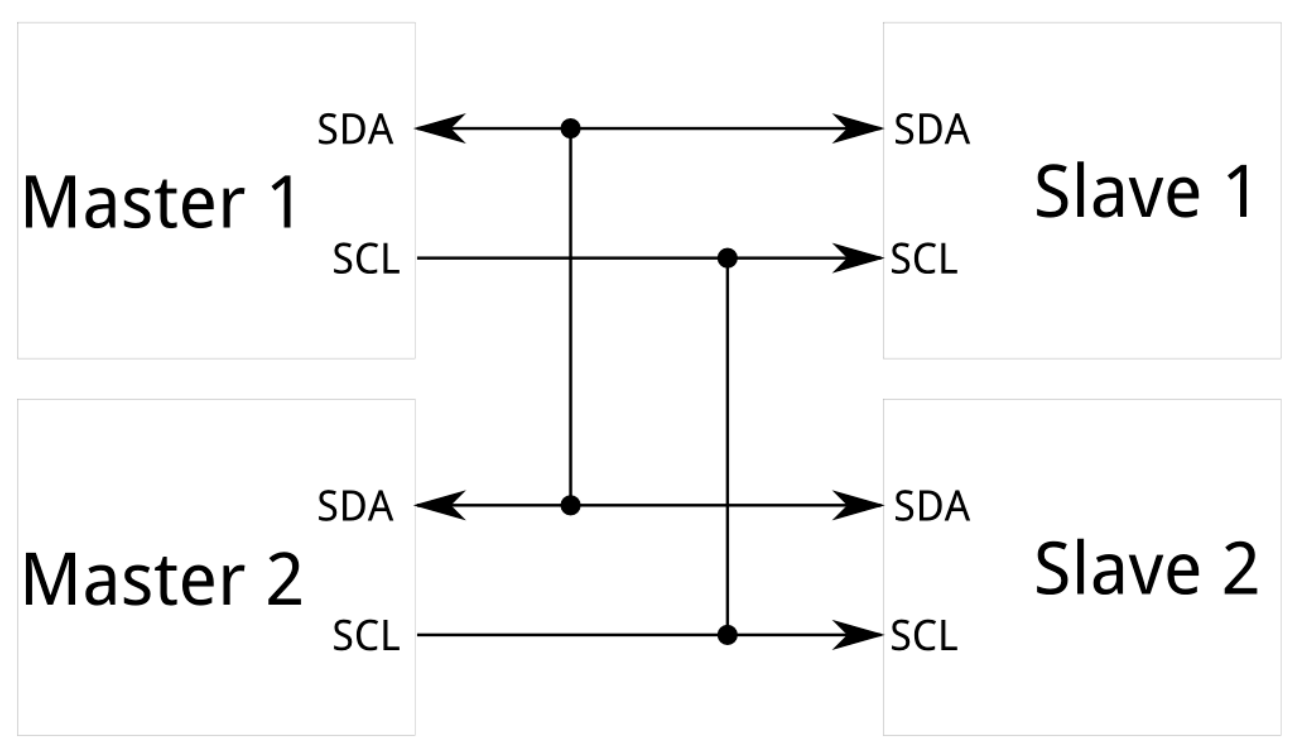
\includegraphics[width=0.6\textwidth]{./images/chapter3/i2c.png}
	\caption{I2C}
	\label{fig:i2c}
\end{figure}

\subsubsection{SPI}
\label{subsubsec:SPI}

Το \textit{Serial Peripheral Interface} (\textit{SPI}) αναπτύχθηκε από τη Motorola\footnote{\url{https://www.motorola.com/us/}} και αποτελείται από τους ακόλουθους διαύλους:

\begin{itemize}
	\item MOSI: Master Out Slave in
	\item MISO: Master In Slave Out
	\item SS: Slave Select
	\item SCLK: Serial Clock
	\item Ακριβής χρονισμός
\end{itemize}

Μια αναπαράσταση των διαύλων μπορούμε να δούμε στο \autoref{fig:spi}. Όπως το I2C, έτσι και το SPI είναι πρωτόκολλο επικοινωνίας master-slave. Στο SPI, πρώτα η master συσκευή διαμορφώνει το ρολόι σε μια συγκεκριμένη συχνότητα. Επιπλέον ο δίαυλος SS χρησιμοποιείται για την επιλογή του κατάλληλου slave. Αφού επιλεγεί η slave συσκευή, αρχίζει η επικοινωνία.

\begin{figure}[!ht]
	\centering
	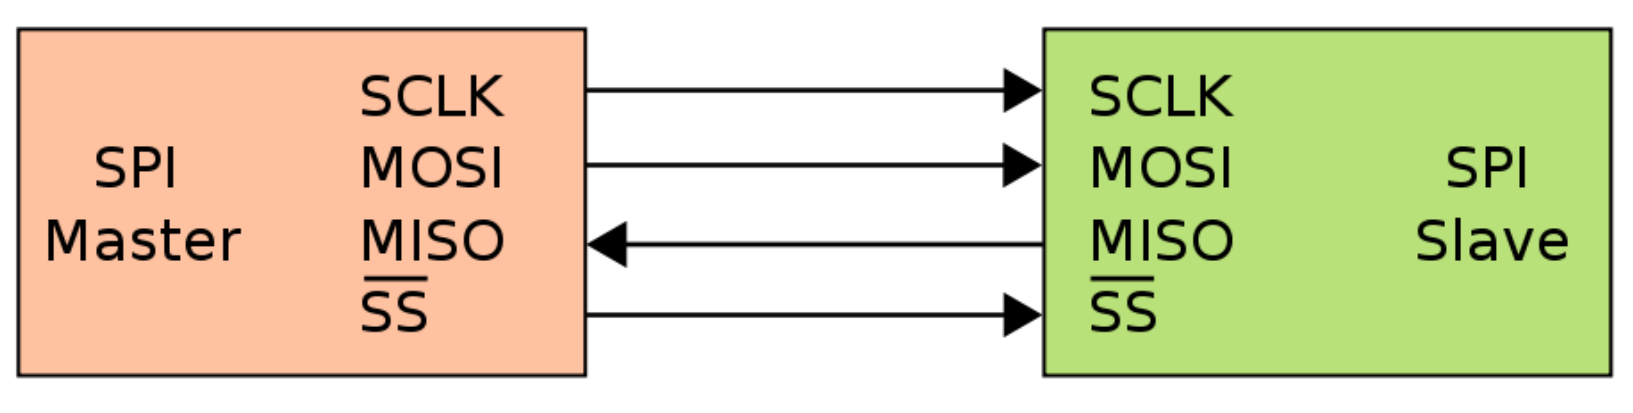
\includegraphics[width=0.8\textwidth]{./images/chapter3/spi.png}
	\caption{SPI}
	\label{fig:spi}
\end{figure}

\subsubsection{UART}
\label{subsubsec:UART}

Το \textit{Universal Asynchronous Receiver/Transmitter} (\textit{UART}) δεν είναι ακριβώς πρωτόκολλο αλλά ένα φυσικό κομμάτι υλικού που μετατρέπει παράλληλα δεδομένα σε σειρειακά. Ο κύριος σκοπός του είναι η μετάδοση και λήψη δεδομένων σειριακά.

Αποτελείται από δύο διαύλους έναν για την αποστολή των δεδομένων και έναν για τη λήψη. Επομένως χρειάζεται δύο ακροδέκτες, ο Rx (δέκτης) και ο Tx (πομπός), το οποίο φαίνεται και στο \autoref{fig:uart}).

Το UART μεταδίδει δεδομένα ασύγχρονα, άρα κάνενα σήμα ρολογιού δεν σχετίζεται με τη μετάδοση και τη λήψη δεδομένων. Αντί για σήμα ρολογιού, χρησιμοποιεί bit έναρξης και διακοπής μέσω πραγματικών bit δεδομένων, τα οποία καθορίζουν την έναρξη και το τέλος του πακέτου δεδομένων.

\begin{figure}[!ht]
	\centering
	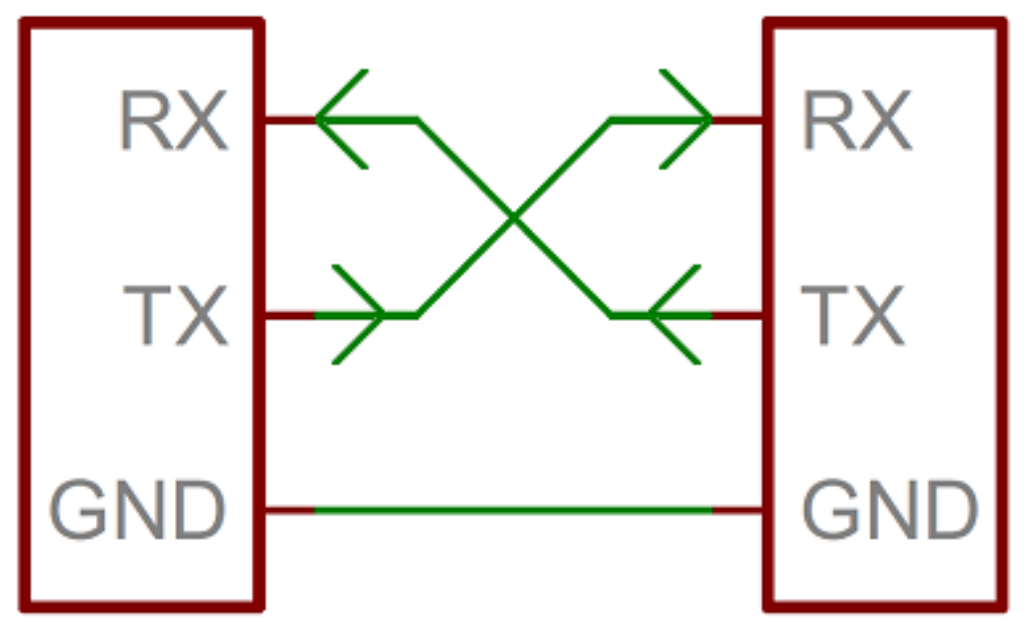
\includegraphics[width=0.5\textwidth]{./images/chapter3/uart.png}
	\caption{UART}
	\label{fig:uart}
\end{figure}